\chapter{SQL -- Einführung}
\renewcommand{\chaptertitle}{SQL -- Einführung}

\lehead[]{\sf\hspace*{-2.00cm}\textcolor{white}{\colorbox{lightblue}{\makebox[1.60cm][r]{\thechapter}}}\hspace{0.17cm}\textcolor{lightblue}{\chaptertitle}}
\rohead[]{\textcolor{lightblue}{\chaptertitle}\sf\hspace*{0.17cm}\textcolor{white}{\colorbox{lightblue}{\makebox[1.60cm][l]{\thechapter}}}\hspace{-2.00cm}}
%\chead[]{}
\rehead[]{\textcolor{lightblue}{AvHG, Inf, My}}
\lohead[]{\textcolor{lightblue}{AvHG, Inf, My}}


\section{Relationale Datenbanken -- Überblick}

\subsection{Relationale Datenbanken}

Daten können auf verschiedene Arten strukturiert abgespeichert werden, z.B.
könnte man die Daten nach einem Index ordnen oder in einer Baumstruktur geordnet
ablegen. Für große Datenmengen hat sich heutzutage das \emph{relationale
Datenmodell} durchgesetzt, bei dem die Daten in Tabellen abgespeichert werden.
\textit{Relation} ist eine mathematische Bezeichnung für eine Tabelle.
Daher der Name relationale Datenbanken. Ein Programmierer kann nicht nur die
Daten einzelner Tabellen abfragen. Relationale Datenbanksysteme besitzen auch
die Fähigkeit Tabellen zu verknüpfen und auf diese Weise komplexere
Informationen zu generieren. Nahezu alle bekannten Datenbanksysteme arbeiten
heute nach dem relationalen Modell.

\subsection{Datenbanksysteme}

Computerprogramme zur Beschreibung, Speicherung und Wiedergewinnung von umfangreichen
Datenmengen nennt man Datenbanksysteme. Bekannte Datenbanksysteme sind:

\begin{compactitem}
  \item Oracle
  \item DB2
  \item MySQL
  \item MS SQL Server
  \item PostgreSQL
\end{compactitem}

Die Software innerhalb eines Datenbanksystems, welche die Eingabe, Verwaltung
und Ausgabe von Daten ermöglicht, nennt man \emph{Datenbankmanagementsystem
(DBMS)}.

\subsection{Organisation eines Datenbankmanagementsystems (DBMS)}

\begin{figure}[h]
  \centering
   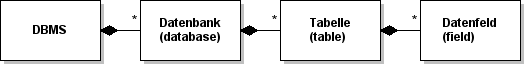
\includegraphics[width=0.60\textwidth]{./inf/SEKII/32_SQL_Einfuehrung/DBMS}
   \caption{UML-Klassendiagramm eines DBMS}
   \label{fig:dbms}
\end{figure}

Ein Eintrag in der Tabelle, der genau zu einer Zeile und einer Spalte gehört,
heißt \textit{Datum} (Einzahl von Daten) oder \emph{Datenwert}. Die Datenwerte
in einer Zeile der Tabelle bilden zusammen einen \emph{Datensatz} (engl.\
record).

\subsection{Terminologie}

Wir werden im Unterricht von Datenbanken, Tabellen, Spalten und Zeilen sprechen,
parallel dazu aber auch einige andere Begriffe verwenden. Und wer sich anderswo
über Datenbanken informiert, wird dann oft noch weitere Begriffe finden. Welche
Begriffe als Synonyme benutzbar sind zeigt die folgende Tabelle:

\begin{center}
\bgroup
\def\arraystretch{1.2}
\begin{tabularx}{0.75\textwidth}{|X|p{60mm}|}\hline
%\begin{tabular}{|l|l|l|}\hline
\textbf{hier hauptsächlich verwendet} & \textbf{Synonyme} \\ \hline 
Datenbank & Schema \\ \hline 
Tabelle & Relation, Entitätstyp, Klasse \\ \hline 
Spalte & Attribut, Feld \\ \hline
Zeile & Datensatz, Entität, Tupel, Objekt \\ \hline
\end{tabularx}
\egroup
\end{center}

\subsection{Front End und Back End}

Der Benutzer kann die Daten eines DBMS auch von einem entfernten Rechner
abfragen ohne zu wissen, wie die Datenbank eigentlich intern aufgebaut ist. Die
Software, die der Benutzer zur Abfrage und Veränderung der Datenbank benutzt,
nennt man \emph{Front End}. Das Front End besitzt auch die
Bedienungsoberfläche, die der Benutzer sieht. Das DBMS, das sich unter Umständen
auf einem ganz anderen Rechner befindet, wird dagegen auch als \emph{Back End}
bezeichnet. Um mit einem DBMS arbeiten zu können, muss ein Front End immer eine
Verbindung (\emph{Connection}) zu \glqq seinem\grqq\ Back End aufbauen.

\subsection{SQL -- Structured Query Language}

Alle gängigen Datenbank-Front-Ends benutzen die Sprache SQL für die Abfrage und
Manipulation ihres Back Ends. Das Front End sendet an das Back End SQL-Befehle
zur Steuerung des DBMS. SQL ist eine sogenannte \emph{deskriptive Sprache}:
Mit SQL legt man nur fest, was das DBMS tun soll. Wie es das tut, bleibt dem
DBMS überlassen.

Wenn man mit einer Programmiersprache wie z.B.\ Java oder PHP einen
Datenbank-Client programmiert, dann werden die SQL-Befehle zur Steuerung der
Datenbank in die Programmiersprache \glqq eingebettet\grqq , d.h.\
man generiert mit der Programmiersprache SQL-Befehle, die an das DBMS gesendet
werden.
